%!TEX root = ../talk.tex
\chapter{Overview and Comparison of P2P File Synchronization and Storage Solutions}
\markboth{Overview and Comparison of P2P File Synchronization and Storage Solutions}{}
\chaptauthors{Josua Fr\"ohlich, Simon Ruesch}

\Kurzfassung{%
Today, file synchronization and storage is demanded more than ever. The average user owns multiple devices that are continuously connected to the internet and works on the device which is the most practical for his current situation. As a consequence, users require their files to be up-to-date at all times regardless of which device the user wants to access the files on. A second aspect is that there is an ever increasing demand for systems which allow file sharing between users, such that multiple people can work on the same files independently, whether at the same time or not. Traditional cloud based file storage and synchronization systems cover these requirements but also come with drawbacks, mainly with regards to security and availability in case of server faults or attacks. To address these drawbacks, P2P file storage and synchronization systems have been developed
This seminar thesis aims to give an overview over the current available P2P file storage systems and categorize them according to their different aspects. To do this, a set of criteria was determined which which the systems could be compared.
The findings of the thesis show that P2P systems can be an improvement over cloud based systems in security and fault-tolerance aspects but they exhibit problems in other areas as in availability and trust. The examined systems all specialize in a certain aspect and, as a trade-off, are worse in others.
}

\newpage

% the table of contents
\minitoc

\newpage

\section{Introduction and Problem Statement}
Today, file synchronization and storage is demanded more than ever. The average user owns multiple devices that are continuously connected to the internet and works on the device which is the most practical for his current situation. As a consequence, users require their files to be up-to-date at all times regardless of which device the user wants to access the files on. A second aspect is that there is an ever increasing demand for systems which allow file sharing between users, such that multiple people can work on the same files independently, whether at the same time or not.

In general, the existing file synchronization and storage systems can be categorized into two groups: Client-Server based distributed file storage systems (also sometimes referred to as Cloud storage systems) and Peer-to-Peer file storage systems. Since giving a comprehensive treatment to both of those categories would be beyond the scope of this seminar thesis, the focus here lies on Peer-to-Peer file storage systems, henceforth called P2P file storage systems.

This seminar thesis aims to give an overview over the current available P2P file storage systems and categorize them according to their different aspects. In chapter \ref{sec:background} we want to give an impression of the background of peer-to-peer systems including historical aspects, manly predecessor approaches of file storage solutions. Chapter \ref{sec:approach} shows the procedures and approaches used in this thesis to justify the decisions made for the choice of systems to compare and also for the criteria according to which the systems were compared with each other. The four chosen peer-to-peer systems; Storj, AeroFS, Hive2Hive and BitTorrentSync will be described in chapter \ref{comparisons}. The findings will also be summarized on the base of comparing the assets and drawbacks of these systems and by comparison to Dropbox, a popular distributed file storage system.

\section{Background} % @Josua
\label{sec:background}
This section gives a short basic overview over the most important topics concerning P2P systems, file storage, and the special requirements of P2P file storage systems compared to those of traditional and distributed file storage. Also, the most common drawbacks of these older systems compared to peer-to-peer systems is shown.

\subsection{File Storage}
The Free Dictionary defines file storage as follows:
\begin{quote}
A generic term for warehousing electronic files. It may refer to local storage in a PC or tablet or remote storage on the Internet. The primary storage devices are hard drives and solid state drives\cite{thefreedictionary}.
\end{quote}
To begin with an overview of the different approaches for file storage and some historical aspects there are basically three different file storage generations classified. Afterwards it is often talked about distributed file storage (DFS) meaning that file storage is not managed by only one system that is geographically constricted. When talking about cloud a metaphorical synonym for DFS is intended.

Firstly, talking about traditional or \textit{Client-Server file storage}, also called \textbf{1st generation DFS}, systems where the cloud consists of one or multiple huge file server storing all the files of multiple clients being on the same network are opined. The main problem in such systems is the file server itself acting as a \textit{single point of failure} and thus becomes a \textit{bottleneck}, illustrated in figure \ref{1st_gen_dfs}.
	\begin{figure}[H]
		\begin{center}
		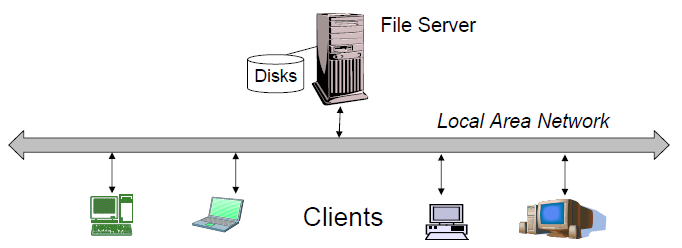
\includegraphics[scale=0.25]{Talk5/1st_gen_dfs.PNG}
		\end{center}
		\caption{1st Generation DFS \cite{wikimedia:p2p}}
		\label{1st_gen_dfs}
	\end{figure}
\textit{Distributed file systems} known as \textbf{2nd generation DFS}, not to be confused with distributed file storage, show some similarities to the traditional system except files being stored on a cluster of servers, so each server stores parts of the original files. In general RAID (Redundant Array of Independent Disks) is used to hopefully avoid storage medium failure and enhance data throughput. These systems are known to be symmetric and scalable. Scalable is an indicator for how easy it is to add endpoints to a system. Figure \ref{2nd_gen_dfs} shows an scheme of a distributed file system.
	\begin{figure}[H]
		\begin{center}
		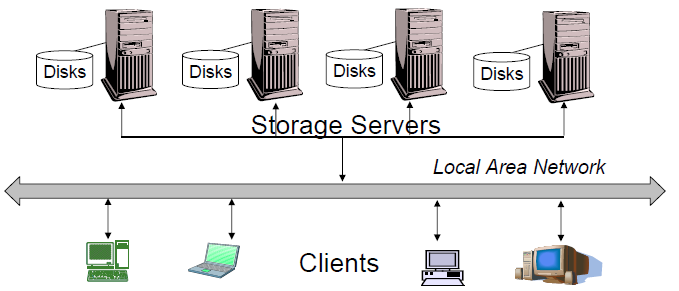
\includegraphics[scale=0.25]{Talk5/2nd_gen_dfs.PNG}
		\end{center}
		\caption{2nd Generation DFS}
		\label{2nd_gen_dfs}
	\end{figure}
The \textbf{3rd generation DFS}, namely \textit{peer-to-peer systems} in general do not have such a clear structure and separation between clients and servers. Each peer, also called node, which means each device connected to the network being able to store or access data on that network is connected to other peers, see figure \ref{3rd_gen_dfs}. The whole system is self-organizing, autonomous and heterogeneous. Heterogeneity in the sense of what systems are within such a network and what bandwidth rate is available, meaning it does not matter whether a node is a powerful server on broadband or a mobile device on it's mobile network. Autonomy and self-organization is the basic principle and indicator for P2P systems and describes the process how other peers can be discovered and how the network itself sets up. Peers can give access, read and or write to other peers to specific files and folders, and as long as the peers providing the data are connected to the network the files are accessible.
	\begin{figure}[H]
		\begin{center}
		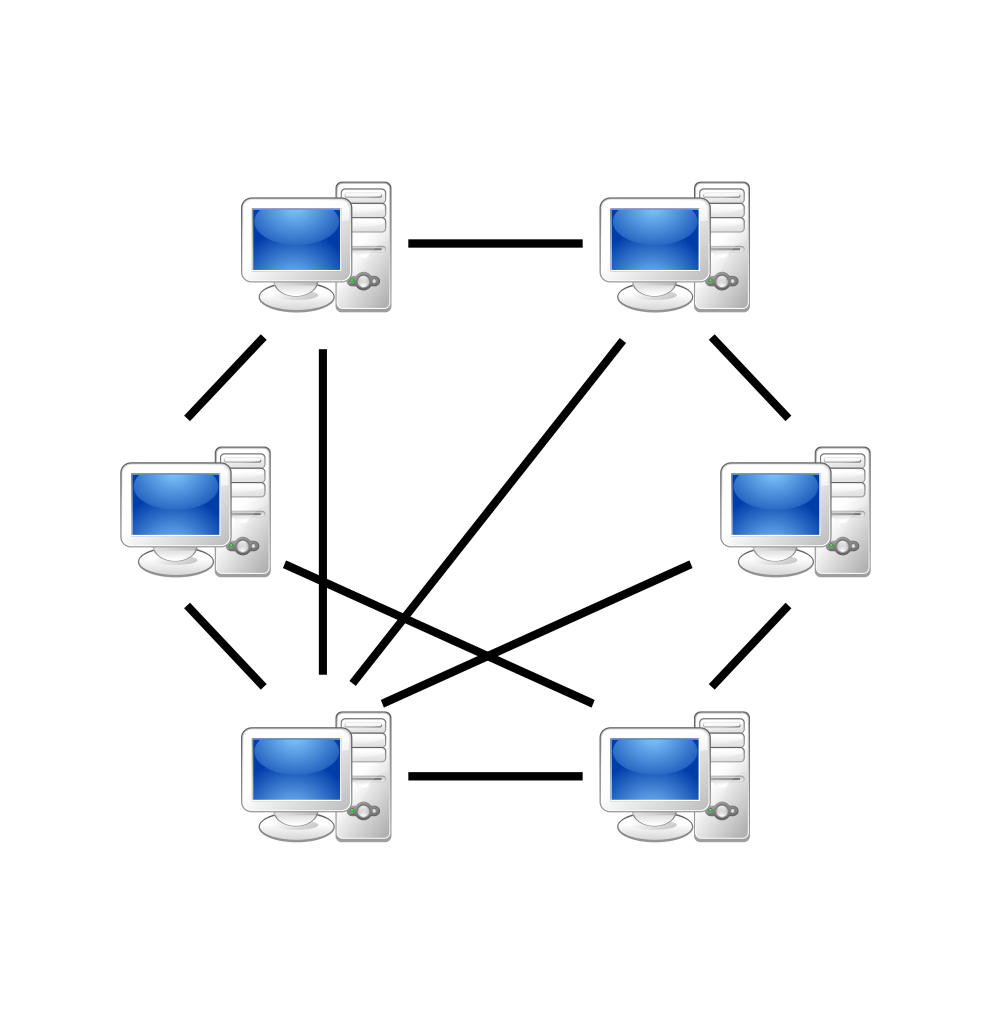
\includegraphics[scale=0.25]{Talk5/3rd_gen_dfs.PNG}
		\end{center}
		\caption{3rd Generation DFS \cite{wikimedia:p2p}}
		\label{3rd_gen_dfs}
	\end{figure}
As each approach of distributed file storage may have his benefits there is no system without drawbacks or even constraints. This is one of the main reasons why first and second generation DFS are still omnipresent, but peer-to-peer technology is on the increase as technology progresses and acceptance and mistrust of society disappears.

\subsection{Peer-to-Peer}
In this section a deeper understanding of the main ideas and goals of Peer-to-Peer systems will be given. Though it is not possible to go very deep in this topic, the idea is to give an overview and a basis for the related work in following sections. First of all a very detailed definition of what Peer-to-Peer systems can be described as is given. Later it is explained what type of peering scheme exist and in the end a summary of the well known assets and drawbacks of peer-to-peer systems compared to traditional cloud storage is done.
\begin{quote}
A distributed network architecture may be called a Peer-to-Peer (P-to-P, P2P,...) network, if the participants share a part of their own hardware resources (processing power, storage capacity, network link capacity, printers,...). These shared resources are necessary to provide the Service and content offered by the network (e.g. file sharing or shared workspaces for collaboration). They are accessible by other peers directly, without passing intermediary entities. The participants of such a network are thus resource (Service and content) providers as well as resource (Service and content) requestors (Servent-concept)\cite{ptp:definition}.
\end{quote}
The goal behind P2P systems is to move away from the traditional client-server architecture to get as far away from their drawbacks as possible. Instead of having one machine acting as a server only answering requests by clients when these clients send those requests, in P2P, the roles of the client and server are combined into one machine (hereforth called peer). Peers then can form a network of peers, i.e., a peer-to-peer network.

There are some well-known advantages and disadvantages in peer-to-peer systems. As for traditional distributed file storage the server can become the single point of failure and RAID networks are expensive and sophisticated to maintain whereas peer-to-peer networks do not have to deal with all of these problems. P2P systems naturally are scalable and excellent in fault tolerance what needs to be archived heavy-going for centralized systems. However, peer-to-peer systems are quite difficult to manage and good security is hard to achieve but having these concerns controlled by a single instance like it is for centralized systems, it is easy to obtain \cite{tomp2p:p2p_introduction}.

Generally, four different types of P2P networks are classified. Mostly it is not possible to clearly associate a known system to only one of these four basic approaches because most systems on the market do not provide such a clear structure or use multiple approaches. Nonetheless usually one approach sticks out \cite{ptp-introduction:tomptp}.
\begin{enumerate}
	\item \textbf{Centralized P2P} as indicated in figure \ref{centralized_p2p} shows similarities to the classical client-server model where peers in fact communicate directly with each other but with the help of a central server. A good known service as an example for centralized P2P is Napster which uses central peer serves as directories. AeroFS, one of the systems later in detail discussed uses a similar approach too.
	\begin{figure}[H]
		\begin{center}
		
\includegraphics[scale=0.2]{Talk5/centralized_p2p.PNG}
		\end{center}
		\caption{Centralized peer-to-peer}
		\label{centralized_p2p}
	\end{figure}
	\item \textbf{Hybrid P2P} provides so called \textit{super peers} to find other peers and resources. Peers communicate to these super peers until the resource is found and thus the peers can communicate directly. This paper does not cover any detailed discussion of a hybrid system but a well known service is for example Sykpe. Figure \ref{hybrid_p2p} illustrates a hybrid approach:
	\begin{figure}[H]
		\begin{center}
		
\includegraphics[scale=0.2]{Talk5/hybrid_p2p.PNG}
		\end{center}
		\caption{Hybrid peer-to-peer}
		\label{hybrid_p2p}
	\end{figure}
	\item \textbf{Pure P2P} systems, also known as \textit{unstructured P2P} systems are systems where all peers are equally powerful communicating without any server or super peer, so peers communicate directly and act as relays to find demanded resources. BitTorrentSync and Storj, both systems that will be discussed in detail in a moment are systems which use a pure P2P approach as shown in figure \ref{pure_p2p}:
	\begin{figure}[H]
		\begin{center}
		
\includegraphics[scale=0.2]{Talk5/pure_p2p.PNG}
		\end{center}
		\caption{Pure (unstructured) peer-to-peer}
		\label{pure_p2p}
	\end{figure}
	\item \textbf{Structured P2P} as shown in figure \ref{structured_p2p} are similar to pure P2P however the peers are organized in a specific structure, e.g. a tree, often a DHT which is used to enhance peer and resource detection. A DHT is just like a normal hash table where hashes of the keys are stored and these keys indicate on which peer the requested files are. Each peer is responsible for a specific key range and henceforth is called \textit{distributed hash table}.
	\begin{figure}[H]
		\begin{center}
		
\includegraphics[scale=0.2]{Talk5/structured_p2p.PNG}
		\end{center}
		\caption{Structured peer-to-peer}
		\label{structured_p2p}
	\end{figure}
\end{enumerate}

Peer-to-peer networks often lack of having enough peers continuously connected to the network. Where peers are defined as some volunteers helping for important files enable fast transfer speed.

\subsection{Problems of Common Synchronization and Sharing Services}
File synchronization has do address and deal with several problems. Depending on the type of file storage and synchronization that is used, some problems might be easy to address and some are even impossible to fully cover. In traditional file storage for example the main problem is the server itself which becomes a bottleneck and is vulnerable to targeted attacks e.g. DDOS (distributed denial of service) attacks. Private data on these large, external data centers is often not encrypted or if it is, the keys are stored on the same server too, as will be shown later in the example of Dropbox. Users do not have control over who can access their private data and he or she is bound to the respective pricing and terms of the service. Such systems often lack of version control and conflict management \cite{hive2hive}.

Depending on the peering scheme used: e.g. manageability gets more complicated as it is for pure P2P and availability is downscaled in centralized P2P where the server again becomes a bottleneck. But for all peering schemes trust is a big talking point. As it is proven to successfully undermine powerful and well secured servers it is just a logic implication that for peers, which represent normal household computational devices, manipulation must be much simpler.

\section{Approach} % @Simon
\label{sec:approach}
In this section, our reasons and a justification for the chosen systems is provided. Additionally, the criteria we chose to classify the different file storage systems are listed and stated below.

\subsection{Justification of the chosen systems}
During research discovering so many peer-to-peer systems a selection of a few of them was inevitable. The criteria that were chosen for evaluation were:
\begin{enumerate}
\item \textbf{Availability and maturity} -- \textit{Is the system currently available and are the concepts developed and implemented and not only ideas?}\\
We required there to be good documentation or papers of the systems to be able to cover as many criteria as possible.

\item \textbf{Academic or commercial release} -- \textit{Was or is the system being developed for academical and research purposes or is the system available commercially?}\\
We wanted to have a good mixture of academical and commercial systems.

\item \textbf{Importance in future} -- \textit{Does the system show aspects, meaning well-written functionalities which indicate that it might play an important role in future?}\\
Admittingly hard to estimate, this criteria was chosen to select systems that we expect to be around for the next few years.
\end{enumerate}

\subsection{Criteria}
The decision of criteria was made to fit what we feel are the most important aspects that a prospective user considers before making the decision of which file storage system to use. The following criteria were chosen for classification and a justification for each choice is given.

\begin{enumerate}[(a)]
\item \textbf{Peering Scheme} -- \textit{How are peers connected, where is user data stored, how do users communicate and what messages do they exchange?}\\
This classification criteria describes the technical aspects of the peer-to-peer system. As described in Section \ref{sec:background} there are many different forms of peering schemes for peer-to-peer networks. It also may be important for users to know how and where their data is physically stored in the network. Some users may be weary of storing their personal data on the machine of a stranger, even if the data is divided into chunks and encrypted. This aspect also deals with how peers can share data with each other and which communication possibilities exist. 

\item \textbf{Encryption} -- \textit{Are the communication between peers and the files stored encrypted and with which algorithm?}\\
Users tend to give great importance to the fact that their personal data can only be read by authorized peers. Therefore, a strong encryption mechanism is almost mandatory. This criteria analyzes if and how the users' files and their communication with other peers is encrypted.

\item \textbf{Trust and Integrity} -- \textit{How is trust established between peers? How are files and communication protected against fraudulent users and attacks?}\\
This criteria analyzes how a peer can check if their communication peer is who he or she claims to be and therefore if that peer can be trusted. Secondly, this criteria looks at how users can verify the integrity of their files as in, if there haven't been any malicious changes to them.

\item \textbf{Payment Scheme} -- \textit{Is the system free or paid? Who gets paid what under which circumstances?}\\
Of course, a user is more likely to use a system the cheaper it is. However, there is also the possibility for users to earn money by using the system, e.g., by offering up their excess storage space.

\item \textbf{Fairness} -- \textit{How is the workload distributed in the system especially considering the heterogeneous hardware used by the peers?}\\
With this criteria, we want to check if a system distributes the workload of file storage equally among the peers, such that not a single peer is storing all files of all peers. It is obviously undesirable for a peer to take part in a system where it has a large workload compared to the benefit gained. Also, an uneven distribution can lead to the problem of single points of failure.

\item \textbf{Fault-tolerance and Availability} -- \textit{How does the system guarantee that files are available to the users at all time?}\\
The system should handle network failures and prevent data loss when a peer just shuts off the network. Users are impatient and do not want to wait for hours until they can access their data otherwise they probably will drop the system and look for a better solution.

\item \textbf{Type of Distribution} -- \textit{Is the system only a library or a dedicated software client?}\\
This aspect determines the ease of use of the system, but also if a expert user can build his or her own application on top of the provided system.

\item \textbf{Source code availability} -- \textit{Is the system open-source or closed source?}\\
This aspect is most relevant to application developers but might also be of interest for conventional users. If a system is open source, an application developers can make changes to the program code and may also contribute to future releases of the system. However, this can also be detrimental. Programmers may be able to change certain parts of their application which in turn may bypass security and fairness concepts normally applied in the system. For example, it might be possible for a malicious programmer to disable storage of data from other users while he or she stores large amounts of data of their own on other peers. In a different, more extreme example, a malicious programmer can commit changes to the public source code that contains backdoors to the encryption algorithms, allowing the programmer to access files which he or she is not normally authorized to access. The feasibility of this example depends on how many people are involved with the development of the open source project and how skilled the owners of the code are at detecting such malicious changes.
Closed source code can also be disadvantageous. If the source code is not accessible, users have to trust the developer that the security algorithms are properly implemented and that their data is only accessible to authorized parties. With open source code, an adept user can at all times verify the quality of the security scheme. Also, the more developers that are actively working on the open source project and verifying commits, the smaller is the possibility of malicious code sneaking in.

\item \textbf{User base} -- \textit{How many users does the system currently have? Is the system intended for businesses or private users?}\\
Firstly, the amount of users already using the system may be an indication of the quality of the system to prospective users. Also, there exists the network effect which may make it more useful for users to use a system which is already widely established instead of one which is only used by few people. Additionally, an open source system with many active users and developers may be more secure than ones with a smaller install base. However, a larger user base also makes the system a more desirable target of attack for malicious users. Secondly, the feature set of a system can also be geared more towards business applications instead of private users. It is usually more prudent to choose a system that is more suitable to the goals of the user.

\item \textbf{Status} -- \textit{In what state is the system? Is it available for use, a scientific prototype or canceled?}\\
A system should be available for use or at least available in near future. Digital senescence of systems not used anymore should not be underrated also since data storage is often not meant to last only for a few months or years. Scientific prototypes are important to get to know what the current point of technology is able to achieve and thus have a possible view into the future where more systems with such approaches may be used.
\end{enumerate}

\section{Comparisons}
\label{comparisons}
In this section, we classify and compare four exemplary P2P file storage systems according to the classification criteria given in the preceding section. We also compare the P2P file storage to a popular distributed file storage system to find similarities and differences. At the end, highlight the findings in a table comparing the file storage systems with each other.

\subsection{Storj} % @Josua
One can describe Storj (pronounced storage) as a completely decentralized and blockchain-based peer-to-peer cloud storage system with it's major concern on security and efficiency. Being primary launched in July 2014 it further includes a peer-to-peer payment system service similar to Bitcoin \cite{storj:blog:what_is_storj}. Storj mainly consists of two applications, namely DriveShare (also called Driveminer) and Metadisk. The former uses unused hard drive space of users and the latter is a web-service used for file storage and sharing. The main approach of Storj claims that the average user has a lot of unused hard drive space and for many systems a user pays for a specific amount of space even if he or she doesn't use it at all. Storj further claims a user is only obligated to pay for his used space and thus will be much cheaper than any other available cloud storage.

\textbf{Peering scheme:} There are no centralized servers but information of where other shards of a specific file are located is stored in the Storj blockchain. In the blockchain itself no files but only meta-data (file hashes) for file lookup are stored. A blockchain is very hard to manipulate as every peer gets a copy of it. Peer discovery is done by an advertisement system whose functionality is not explained in precision \cite{storj:PDF}. Storj remains as unstructured peer-to-peer system using the blockchain as reference for file discovery.

\textbf{Encryption:} Before encryption and distribution files are splitted into so called shards. These shards, a multiple of 8 or 32 Bit-sized file chunks, are being added a deterministic salt, then uniquely encrypted and distributed over the network. A farmer, which means a hard drive space providing peer, does not get a whole copy of a file (all necessary shards to compose the original file) but the shards are distributed to multiple farmers. Per default there are at least three redundant copies of a shard all the time available. For enhanced security for sensitive or important data it is also possible to combine shards, e.g. with garbage data or other client's data. The prof of redundancy claims if a node goes offline a copy of all it's shards is made and the shards moved to another node. In addition a user can chose how and with what his files will be encrypted  \cite{storj:PDF}.

\textbf{Trust and Integrity} With the help of a \textit{pseudo-reputation system} like advertisements in peer discovery to get data quality and type by tracking it or directly from the network, evaluations are made to detect and qualify reputable peers. A peer is reputable if it is marked as trustworthy by the algorithm. Storj uses a recommendation system for peers to improve the algorithm \cite{storj:PDF}.

The \textit{proof of storage} via \textit{merkle audits}, also audits through \textit{hash challenge} ensure whether a farmer is able to proof he holds a specific file, or more precise; a specific shard and that the shard has not been changed or maliciously modified by anyone or anything. A merkle tree is a hash tree where every non-leaf node is labeled with the hash of the labels of its children nodes, so to ensure whether a child is correct it is sufficient to ensure whether the parent node has a correct hash.

Storj uses different so called \textit{heartbeats} to check whether a file is correctly shattered and stored. Shards are furthermore split into pieces and checked for fulfillment of the security requirements and modification detection through heartbeats as shown in figure \ref{storj_heartbeat}. A \textit{full heartbeat} means the whole shard integrity is checked but this is shown to be very I/O inefficient whereas \textit{cycle heartbeats} need \textsl{n} heartbeats to generate a full heartbeat. Deterministically generate reads on a shard using a root seed is the third variant for those audits (\textit{cycle heartbeat}), but Storj uses a mixed methodology to improve efficiency.

	\begin{figure}[ht]
		\begin{center}
		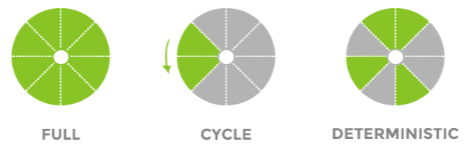
\includegraphics[scale=0.8]{Talk5/storj_heartbeat.PNG}
		\end{center}
		\caption{Heartbeat shard audit \cite{storj:PDF}}
		\label{storj_heartbeat}
	\end{figure}

But what happens if a malicious farmer knows the decryption key of a specific file? He won't be able to complete the audits (heartbeats) for all shards since he isn't assigned to all of them. In addition this leads to the \textit{prove of redundancy} of particular shards which means that each copy of a shard is unique \cite{storj:PDF}.

\textbf{Payment scheme:} On DriveShare users, the so called farmers, can lease their unused available hard drive space and get paid for this service in Storjcoin X (SJCX), that is based on Bitcoin. SJCX rewards, depending on the current crowdsale phase, are between 38'500 and 32480 SJCX per Bitcoin\cite{storj:crowdsale}. Users of Metadisk will pay bitcoin (BTC) for these hard drive space to be able to share their files.

\textbf{Fairness:} Storj has no central devices and through the \textit{Proof-of-Redundancy} it is guaranteed that the files are evenly distributed. Also prices can vary on the base of bandwidth speed and location of the peer and type of hardware provided \cite{storj:PDF}.

\textbf{Fault-tolerance and Availability:} To default there are thee copies of a shard all times accessible which means a shard gets copied to another node if a node goes offline. The user can request more copies in exchange of money. In this way, if a node fails an audit or is unreachable, the \textit{network replication process} is initiated and thus the network is able to 'heal' itself.

To archive accordance of file location and integrity over the whole network a blockchain like Bitcoin according to Satoshi Nakamoto \cite{bitcoin} is used. The following citation illustrates the basic principle behind a blockchain:

\begin{quotation}
To use a basic analogy, it is easy to steal a cookie from a cookie jar in a secluded area, but it is hard to do so when the jar is instead located in the middle of a public square, being observed by thousands of people \cite{storj:PDF}.
\end{quotation}

\textbf{Type of distribution:} As mentioned above Storj consists of two applications; DriveShare and Metadisk.

\textbf{Source code availability:} Both applications (and even more Storj applications) are fully open-source \cite{storj:github}.

\textbf{User base:} There is no official up-to-date data, in addition the system is currently in beta-phase. The forum of Storj has over one thousand members \cite{storj:forum} and lets assume that there are currently even more storj users. In June 2014 Storj had about more than 3'000 users \cite{storj:crowdsale}.

\textbf{Status:} Storj is currently in beta phase and already available for use. There are three different test groups; A, B and C each with different conditions in terms of a rewarding system, requirements and the starting date. The official launch and avery change in beta phase is planned when a specific amount of SJCX in total has been earned \cite {storj:earlyaccess}.

\subsection{Hive2Hive} % @Simon 
Hive2Hive \cite{hive2hive}, formerly known as Box2Box, is an open source peer-to-peer file sharing and synchronization library that started out as part of a course challenge task project and was further improved in a graduate student's project at the Communication Systems Group at the University of Zurich \cite{hive2hive:about}. It is built on top of the TomP2P library (an open source Distributed Hash Table (DHT) based key-value store) which was also developed at the Communication Systems Group \cite{tomp2p}.

\textbf{Peering Scheme}
A structured P2P peering scheme based on the TomP2P DHT is used. Each peer is assigned an id which signifies for which key space the peer is responsible for storage. For each piece of data that is to be stored in the DHT, an id is generated that shows at which the file is stored. Those ids are generated with a hash function that hashes a certain piece of information that is only known by authorized peers. That means that only peers who have the correct permission have that piece of information and therefore can access that data.
The central piece of data for a user is its user profile, which is stored with a hash of the password and pin of an user. Those are generated when first registering to the system and have to be kept secret from any other peers. The user profile contains the encryption keys of the user and also the file tree, which is a replica of the local file system of the user which holds the files that are stored in the system. The file tree consists of file indexes which represent individual files, each containing the id of a metadata object. These metadata objects are separately stored in the DHT and contain the ids of the file chunks. Before storage, files are divided into chunks, a random id is generated for each chunk and stored in the metadata file of that file. A file chunk is stored at the peer with the id closest to the hashed id of the chunk.

\textbf{Encryption}
Hive2Hive uses a hybrid encryption mechanism for files stored in the DHT. AES-256 is used for symmetrical encryption and RSA with 2048 bit keys is used for asymmetrical encryption. Messages between users are encrypted asymmetrically with a different set of RSA keys.
The keys are stored in the user profile stored in the DHT, which is only accessible by the user which the profile belongs to.

\textbf{Trust \& Integrity}
There are two types of file access permission that can be given to other peers, read access and read/write access. Peers without any of those permissions cannot access a file. File chunks are signed with an MD5 hash to guarantee integrity. Peers have to verify the identity of the peers that they want to share files with themselves.

\textbf{Payment Scheme}
Hive2Hive is open source and is like most open source software free of charge to use.

\textbf{Fairness}
Since ids for file chunks are generated randomly, the file chunks are distributed equally between all peers in the long run. However, there is nothing that prevents peers from storing an extraordinary amount of files

\textbf{Fault-tolerance and Availability}
By default, file chunks are replicated 3 times but higher amounts can be configured.

\textbf{Type of Distribution}
Hive2Hive itself is a library that provides the functionality of file sharing and synchronization. However, an end-user GUI application called Peerwasp \cite{peerwasp} is currently in development that uses Hive2Hive as a basis.

\textbf{Source code availability}
The source code of Hive2Hive, TomP2P as well as Peerwasp is freely available on Github \cite{hive2hive:github}, \cite{tomp2p:github}, \cite{peerwasp:github}. 

\textbf{User base}
Since Hive2Hive is distributed as a library and the developers don't provide an official number, the user base is hard to estimate.

\textbf{Status}
Mature library with active development.

\subsection{BitTorrent Sync} % @Simon
Sync is a peer-to-peer file synchronization system developed by BitTorrent, the company that also developed the famous BitTorrent peer-to-peer protocol for file sharing. Development for Sync started in 2013 and Sync officially left beta in March 2015.

\textbf{Peering Scheme}
In Sync, users do not enter a large static network per se. Rather, connections between peers are established as soon as they start sharing folders with each other. To share a folder, the user can generate a link to it through the software. This link has to be distributed out of band, e.g., through email to the person to share the folder with. The link has to be kept a secret between the peers, since it contains the encryption key of the folder. Also, the link contains a so-called shareID which is unique for each folder and is used to advertise who can access a given folder in the Sync system. There are four different possibilities of peer discovery, i.e., finding out the IP address of a peer: Firstly, if the IP address of the peer is known to the user, it can be entered manually. Secondly, a DHT is in place that can be queried for the shareID and returns the IP address of the authorized peers. Thirdly, there are tracker servers that store a shareID / authorized peers IP address mapping table. Lastly, peers can advertise their shared folders in the LAN through multicast. Any user is free to decide which combination of peer discovery he or she wants to use.

\textbf{Encryption}
Sync uses AES-128 encryption for files while they are in transit. Additionally, the X.509 protocol and SSL are used to encrypt communication between peers.

\textbf{Trust \& Integrity}
The trust in Sync depends on the discretion of how the link to the shared folders is distributed. Users have to be careful that they only provide the link to people that they know are trustworthy. However, Sync also allows users to give their peers either only read access or full read/write access to folders.

\textbf{Payment Scheme}
Sync is available as a free version, but there is also a paid version for 39.99 euros per year that allows users to have an unlimited number of folders among other benefits.

\textbf{Fairness}
The fairness criteria is not applicable to Sync, since files are only shared between a few select peers and they then receive a full copy of the file, therefore all peers store all shared files.

\textbf{Fault-tolerance and Availability}
Since the files are only synchronized between a few trusted peer, one of those peers has to be online for a new peer to enter the synchronization and access the files. The system is fault-tolerant in terms of peer discovery as described above.

\textbf{Type of Distribution}
Sync is available as a desktop application as well as as an application for mobile phones.

\textbf{Source code availability}
BitTorrent Sync is currently closed source.

\textbf{User base}
The latest known number from 2014 claims a user base of 10 million users.

\textbf{Status}
As of March 2015, Sync is fully released to the public.

\subsection{AeroFS} % @Josua
AeroFS is a dedicated software client from Air Computing providing basic peer to peer solutions but some advanced functionality concerning advanced security and encryption, error and data loss prevention and intends to provide the service for low costs. AeroFS is mainly targeted towards business users and companies who need a secure file backup and synchronization service \cite{aerofs}. AeroFS in addition claims to be the 'peer-to-peer version' of Dropbox.

\textbf{Peering scheme:} AeroFS uses a centralized solution as peering scheme but let's the user chose how this will be managed. Air Computing provides two different cloud options and an additional addon, the Team Server:

\begin{enumerate}
\item \textbf{Private Cloud}: Provides private Web Administration, the AeroFS Appliance which is a lightweight virtual machine to manage registration and authentication of users and private Certificate Authority (CA) to manage the AeroFS public key infrastructure (PKI) for client applications.
\item \textbf{Hybrid Cloud}: Supplies a centrally managed file sharing platform for the employees; registration, authentication and user management is done outside the network by AeroFS.
\item \textbf{Team Server} (optional Addon): Lightweight client to enable backup of files and 24/7 availability \cite{aerofs:cloud_types}. But the Team Server again has three different options:
	\begin{enumerate}[(a)]
	\item \textbf{Linked Storage}: Creates a read/write copy of organization's files on the Team Server. Files will still be browseable.
	\item \textbf{Block Storage}: Compresses and de-duplicates files for enlarged disk space. Files won't be browseable anymore.
	\item \textbf{S3 Storage}: Data shared by users of an organization is stored and backed up on Amazon servers compressed and de-duplicated. Files won't be browseable anymore \cite{aerofs:storage_types}.
	\end{enumerate}
\end{enumerate}

\textbf{Encryption:} An \textit{end-to-end encryption} solution is provided, files are encrypted before transaction using AES-256 with 2048-bit RSA and only the recipient is able to decrypt the data transfer \cite{aerofs:security}. The files for syncing itself are eventually stored unencrypted. On the servers of AeroFS are - depending on the solution used - only usernames, the hashes of the passwords and the names of the access authorized users from folders stored (hybrid) \cite{aerofs:security_2}.

\textbf{Trust and Integrity} The amount of users from a borrower is of fixed size (but can grow), also using the AeroFS Applicance as root certificate, no other footprint will be accepted by the clients \cite{aerofs:security}. AeroFS provides three different access permission:
\begin{enumerate}[(a)]
\item Owners (poject administrators): Can add and remove members to the shared folder.
\item Editors: Can create and modify content.
\item Viewers: Can only red content.
\end{enumerate}
A user can manage AeroFS  public key infrastructure (PKI) with his AeroFS Appliance as the root certificate authority (CA). The clients are configured to trust only this AeroFS Appliance which limits the trust footprint. AeroFS also provides an option to remove and wipe data on stolen devices.

\textbf{Payment scheme:} The basic pricing plan (Team) is free up to a user-base size of 30 \cite{aerofs:blog:30_users_free} and the business plan starts above 31 users and according to the size of the user-base the billing is done; a user costs \$15, so e.g. for 40 users the cost totals in \$600, the biggest available size on the website is 1000 users for \$15'000 per month \cite{aerofs:pricing}.

\textbf{Fault-tolerance and Availability:} Multiple users can work on the same file and conflicts are resolved by the users itself by comparing the changes and thus resolve the conflicts. But the AeroFS Appliance and the AeroFS Servers act as single point of failure and no user will be able to register and authenticate anymore.

\textbf{Fairness:} AeroFS provides a load balancer for the AeroFS Appliance which acts as a single API endpoint and securely forwards API requests to running Team Servers and desktop clients. This load balancer thus tries to distribute the workload evenly by maintaining the balance between service availability and data consistency.
If a hard drive gets too full, the versioning systems of the AeroFS Team Server keeps track of the oldest copies and deletes them if the user runs out of space \cite{aerofs:USTO.RE}.

\textbf{Type of distribution:} AeroFS serves a software client and the AeroFS Appliance for users and a admin dash panel for enhanced manageability.

\textbf{Source code availability:} AeroFS is currently closed source but there are some open-source projects on the AeroFS github page.

\textbf{User base:} According to the webpage \cite{aerofs} there are currently around \textbf{50'000\textsc{+}} users.

\textbf{Status:} Available for use and costs-free (depending on type of use).

\subsection{Dropbox}
As comparison to the previously described P2P systems the well-known file hosting service Dropbox that was founded in 2007 will be used as representation for classical cloud storage solutions and measured according to the same criteria. Both, cloud storage and file synchronization are possible with this service with again both, a browser-based and a client application.

\textbf{Peering Scheme:} Dropbox does not use any peer-to-peer technology but rather a client-server system. The data is stored in the Amazon S3 cloud. An accounting system is provided and users can give other users access to their data with either read-only or read and write permission. Folders and files can be shared by link or by username (registration required).

\textbf{Encryption:} Data is stored encrypted with AES-256 and upload and download to the servers can be achieved with SSL. The main critique point is that Dropbox stores the decryption keys on the same servers where the files are stored and thus any administrator has insight into the data.

\textbf{Trust \& Integrity:} There is no mechanism for trust except the user credentials. But as already mentioned, gaining access to the data is no big deal.

\textbf{Payment Scheme:} Dropbox employs a Freemium model where base use is free and more storage can be aquired through a paid subscription.
\begin{enumerate}[(a)]
	\item Dropbox Basic - free - 2 GB
	\item Dropbox Pro - 10 Euro / month - 1 TB
	\item Dropbox for Business - 12 Euro / month - unlimited
\end{enumerate}

\textbf{Fairness:} Fairness is not applicable.

\textbf{Fault-tolerance and Availability:} Dropbox servers act as single point of failure.

\textbf{Type of Distribution:} Available through their website but a GUI application also exists.

\textbf{Source code availability:} Closed source.

\textbf{User base:} Around 300 mio. (29.05.2014)\cite{dropbox:userbase}.

\textbf{Status:} Available for usage.

\section{Summary and Conclusions}
In this section, we provide a summary about the topics mentioned above and draw conclusions about the current state of the available P2P file storage systems and what the future could hold for P2P file storage. The systems chosen are listed among their criteria and compared in a table and finally we will conclude our findings of the research.

\begin{table}
	\centering
		\begin{tabular}{ | *{6}{ p{2.5cm} |} }
			\hline
			& Dropbox & Storj & AeroFS & Hive2Hive & Sync \\ \hline
			Type & Client / Web & Client / Web & Client & Library & Client \\ \hline
			Payment & Free / Paid & Paid & Free / Paid & Free & Free / Paid \\ \hline
			Source Code & Closed & Open & Closed & Open & Closed \\ \hline
			Peering Scheme & None & Unstructured & Centralized & Structured & Pure / Structured / Centralized \\ \hline
			Encryption & Files encrypted, key stored on server & End-End, user defined algorithm & End-End, AES-256 with 2048-bit RSA & Hybrid Encryption for files, Asymmetric for messages & AES-128 for files in transit X.509 and SSL \\ \hline
			Trust and Integrity & No mechanism & Audits (Heartbeats) & AeroFS Appliance / AeroFS Server & Signed messages / Data & Folder links distributed out of band \\ \hline
			User Base & >300 Mio & ~3k & ~50k & Unknown & >10 Mio \\ \hline
			Fairness & Not applicable & Even & Load balancer (Team Server only) & Even & Not applicable \\ \hline
			Fault-Tolerance & Single point of failure & Replication of shards & Copy of each file on each synced device / Backup on Team Server & File chuncks replicated & Copy of each file on each synced device \\ \hline
			Status & Available & Beta & Available & Active development & Available \\ \hline
		\end{tabular}
\end{table}

The results of the research show that peer-to-peer developers have found many different solutions to face the problems that come up when developing and constructing such a system. Thus to simplify implementation there is almost always a specialization of the software for a specific use. To benefit from one aspect of peering scheme it might be inevitable to afford drawbacks and constraints in another aspect. Concrete one could imagine a slider going from e.g. left, Fault tolerance to right, Availability and every developer has to decide where to place his slider between because it is not possible to have them both on 100 percent. Publisher often care about a specific application area, e.g., business use or file synchronization and thus the 'sliders' have to be set as appropriate as possible for every system. Further a clear separation between file synchronization and file storage need to be made. P2P systems are able to do both but depending on the choice of specialization, doing both might no always be as easy.

As a conclusion of the facts described above peer-to-peer systems as well as client-server models do not solve all problems and requirements of file storage and synchronization. One has to always live with some constraints or privacy issues, e.g.: The huge gap between trusting a (well known) storage provider versus a (anonymous) peer. Peer-to-peer does not automatically mean that the single point of failure problem is solved, many P2P systems are not really better than traditional cloud storage systems in this term. The 3rd generation DFS certainly have to deal with some problems traditional client-server models do not, e.g., vulnerability to specialized attacks (e.g., sybil attacks).

\begin{thebibliography}{99}
	\bibitem {aerofs}
		\emph{AeroFS}
		\url{https://www.aerofs.com/},
		March, 2015.

	\bibitem {bitcoin}
		S. Nakamoto:
		\emph{Bitcoin: A Peer-to-Peer Electronic Cash System;}
		\url{https://bitcoin.org/bitcoin.pdf},
		October, 2008.

	\bibitem {bittorrentsync-2}
		J. Farina, M. Scanlon, M. Kechadi:
		\emph{BitTorrent Sync: First Impressions and Digital Forensic Implications;}
		Proceedings of the First Annual DFRWS Europe,
		\url{http://ac.els-cdn.com/S1742287614000152/1-s2.0-S1742287614000152-main.pdf?_tid=10ddb6e2-ce69-11e4-9019-00000aacb35d&acdnat=1426791318_6677afbe19d521d323605261c1d19809},
		Volume 11, Supplement 1, Pages S77\textendash S86, Volume 11, May, 2014.

	\bibitem {box2box}
		A. Lareida, T. Bocek, S. Golaszewski, C. L\"uthold, M. Weber:
		\emph{Box2Box - A P2P-based File-Sharing and Synchronization Application;}
		\url{http://www.csg.uzh.ch/csg/live/teaching/FS13/p2p/challenge/P2P2013DP_017.pdf},
		September, 2013.

	\bibitem {hive2hive}
		\emph{Hive2Hive: Open-Source Library for P2P-based File Synchronization and Sharing;}
		\url{http://hive2hive.com/},
		March, 2015.

	\bibitem {hive2hive:about}
		\emph{Hive2Hive: About Us;}
		\url{https://github.com/Hive2Hive/Hive2Hive/wiki/About-Us},
		March, 2015.

	\bibitem {hive2hive:github}
		\emph{Hive2Hive: Java library for secure, distributed, P2P-based file synchronization and sharing;}
		\url{https://github.com/Hive2Hive},
		March, 2015.

	(https://github.com/tomp2p/TomP2P) (https://github.com/PeerWasp/PeerWasp)

	\bibitem {metadisk}
		S. Wilkinson, J. Lowry:
		\emph{Metadisk: Blockchain-based decentralized file storage application;}
		\url{http://metadisk.org/metadisk.pdf},
		December, 2014.

	\bibitem {p2pfswu}
		C. Wu:
		\emph{Peer-to-Peer Networks;}
		\url{http://www.csie.nuk.edu.tw/~wuch/course/csf641/csf641-04-storage.pdf},
		March, 2015.

	\bibitem {p2pfskangasharju}
		J. Kangasharju:
		\emph{Peer-to-Peer Networks Chapter 4: Peer-to-Peer Storage;}
		\url{http://www.cs.helsinki.fi/u/jakangas/Teaching/P2P/P2P-04-Storage.pdf},
		March, 2015.

	\bibitem {storj:PDF}
		S. Wilkinson:
		\emph{Storj A Peer-to-Peer Cloud Storage Network;}
		\url{http://storj.io/storj.pdf/},
		December, 2014.

	\bibitem {bittorrentsync}
		\emph{Sync;}
		\url{https://www.getsync.com/},
		March, 2015.
		
	\bibitem {storj:blog:what_is_storj}
		\emph{What ist Storj?;}
		\url{http://blog.storj.io/post/87251450053/what-is-storj},
		March, 2015.
		
	\bibitem {storj:deck}
		\emph{Storj - The Crowdsale;}
		\url{http://storj.io/crowdsale.html},
		March, 2015.
		
	\bibitem {storj:crowdsale}
		\emph{Storj Deck - Decentralized Cloud;}
		\url{http://storj.io/Deck.pdf},
		April, 2015.

	\bibitem {storj:github}
		\emph{Storj Labs;}
		\url{https://github.com/Storj/},
		March, 2015.
		
	\bibitem {ptp-introduction:tomptp}
		\emph{TomP2P: A P2P-based high performance key-value pair storage library;}
		\url{http://tomp2p.net/doc/p2p/},
		April, 2015.
		
	\bibitem {storj:forum}
		\emph{Storjtalk;}
		\url{https://storjtalk.org/},
		April, 2015.
		
	\bibitem {storj:earlyaccess}
		\emph{Storj - Early Access;}
		\url{http://storj.io/earlyaccess.html},
		April, 2015.
		
	\bibitem {aerofs:blog:30_users_free}
		Y. Sagalov:
		\emph{AeroFS is now free up to 30 users;}
		\url{https://www.aerofs.com/blog/aerofs-is-now-free-up-to-30-users/},
		April, 2015.
		
	\bibitem {aerofs:pricing}
		\emph{Pricing, AeroFS;}
		\url{https://www.aerofs.com/pricing/},
		April, 2015.
		
	\bibitem {aerofs:peering_scheme}
		\emph{Security Share and Transfer Large Files, Enterprise Solution, Aerofs;}
		\url{https://www.aerofs.com/solutions/transfer-large-files/},
		April, 2015.
		
	\bibitem {aerofs:peering_scheme_2}
		\emph{Flexible Storage for the Enterprise;}
		\url{https://www.aerofs.com/features/flexible-storage/},
		April, 2015.
		
	\bibitem {aerofs:security}
		\emph{Security, AeroFS;}
		\url{https://www.aerofs.com/security/},
		April, 2015.
		
	\bibitem {aerofs:security_2}
		\emph{AeroFS: Das bessere Dropbox? - Golem.de;}
		\url{http://www.golem.de/news/aerofs-das-bessere-dropbox-1304-98485.html},
		April, 2015.
		
	\bibitem {aerofs:storage_types}
		\emph{What Storage Types Can I Use With The AeroFS Team Server? - AeroFS Support;}
		\url{https://support.aerofs.com/hc/en-us/articles/203434524},
		April, 2015.
		
	\bibitem {aerofs:cloud_types}
		\emph{Enterprise Solution - Deployment Options, AeroFS;}
		\url{https://www.aerofs.com/features/deployment-options/},
		April, 2015.
		
	\bibitem {aerofs:USTO.RE}
		Dur\~ao et al:
		\emph{USTO.RE: A Private Cloud Storage Software System;}
		\url{http://www.researchgate.net/profile/Vinicius_Garcia/publication/262284124_USTO.RE_a_private_cloud_storage_software_system/links/5457a3f30cf2cf51648219ed.pdf},
		April, 2015.
		
	\bibitem {wikimedia:p2p}
		\emph{Peer-to-peer;}
		\url{http://en.wikipedia.org/wiki/Peer_to_peer},
		April, 2015.
		
	\bibitem {thefreedictionary}
		\emph{File Storage Definition;}
		\url{http://encyclopedia2.thefreedictionary.com/file+storage},
		April, 2015.
		
	\bibitem {ptp:definition}
		R. Schollmeier:
		\emph{A Definition of Peer-to-Peer Networking for the Classification of Peer-to- Peer Architectures and Applications;}
		\url{http://ieeexplore.ieee.org/xpls/abs_all.jsp?arnumber=990434&tag=1},
		April, 2015.
		
	\bibitem {tomp2p:p2p_introduction}
		\emph{TomP2P, a P2P-based key-value pair storage library}
		\url{http://tomp2p.net/doc/p2p/},
		April, 2015.

	\bibitem {tomp2p}
		\emph{TomP2P, a P2P-based high performance key-value pair storage library}
		\url{http://tomp2p.net},
		April, 2015.

	\bibitem {tomp2p:github}
		\emph{TomP2P, a P2P-based high performance key-value pair storage library}
		\url{https://github.com/tomp2p/TomP2P},
		April, 2015.

	\bibitem {peerwasp}
		\emph{Peerwasp, P2P File Synchronization and Sharing Solution based on Hive2Hive and TomP2P}
		\url{http://www.peerwasp.com/},
		April, 2015.

	\bibitem {peerwasp:github}
		\emph{Peerwasp, P2P File Synchronization and Sharing Solution based on Hive2Hive and TomP2P}
		\url{https://github.com/PeerWasp/PeerWasp},
		April, 2015.
		
	\bibitem {dropbox:userbase}
		\emph{Dropbox Reaches 300M Users;}
		\url{http://thenextweb.com/insider/2014/05/29/dropbox-reaches-300m-users-adding-100m-users-just-six-months/},
		April, 2015.

\end{thebibliography}